\newcommand{\FormalConceptGraph}{%
\begin{tikzpicture}[
    concept/.style={
        circle, draw, minimum size=6mm, inner sep=1mm
    },
    level distance=15mm
]
    
    % Layer 0 (top)
    \node[concept] (n0) {};

    % Layer 1
    \node[concept, below left=15mm and 20mm of n0] (n1) {};
    \node[concept, below=15mm of n0] (n2) {};
    \node[concept, below right=15mm and 20mm of n0] (n3) {};

    % Layer 2
    \node[concept, below left=15mm and 15mm of n1] (n4) {};
    \node[concept, below right=15mm and 15mm of n1] (n5) {};
    \node[concept, below left=15mm and 15mm of n2] (n6) {};
    \node[concept, below right=15mm and 15mm of n2] (n7) {};
    \node[concept, below left=15mm and 15mm of n3] (n8) {};
    \node[concept, below right=15mm and 15mm of n3] (n9) {};

    % Layer 3
    \node[concept, below left=15mm and 10mm of n4] (n10) {};
    \node[concept, below=15mm and 10mm of n4] (n11) {};
    \node[concept, below left=15mm and 10mm of n5] (n12) {};
    \node[concept, below right=15mm and 10mm of n5] (n13) {};
    \node[concept, below left=15mm and 10mm of n6] (n14) {};
    \node[concept, below right=15mm and 10mm of n6] (n15) {};
    \node[concept, below left=15mm and 10mm of n7] (n16) {};
    \node[concept, below=15mm and 10mm of n9] (n17) {};
    \node[concept, below left=15mm and 10mm of n8] (n18) {};
    \node[concept, below right=15mm and 10mm of n8] (n19) {};
    \node[concept, below left=15mm and 10mm of n9] (n20) {};

    % Layer 4 (bottom)
    \node[concept, below=15mm of n10] (n22) {};
    \node[concept, below=15mm of n12] (n23) {};
    \node[concept, below=15mm of n14] (n24) {};
    \node[concept, below=15mm of n16] (n25) {};
    \node[concept, below=15mm of n18] (n26) {};
    \node[concept, below=15mm of n20] (n27) {};
    \node[concept, below=15mm of n11] (n28) {};
    \node[concept, below=15mm of n17] (n29) {};
    \node[concept, below=15mm of n19] (n30) {};

    % Single bottom node
    \node[concept] (n31) at ($ (n22)!0.5!(n30) + (0,-15mm) $) {};
    % \node[concept] (n31) at ($(n22)!0.5!(n30) - (0,15mm)$) {};
    % \node[concept, below=15mm of $(n22)!0.5!(n30)$] (n31) {};

    % Draw downward edges only
    \foreach \from/\to in {
        n0/n1, n0/n2, n0/n3,
        n1/n4, n1/n5, n2/n6, n2/n7, n3/n8, n3/n9,
        n4/n10, n4/n11, n5/n12, n5/n13, n6/n14, n6/n15, n7/n16, n7/n17, n8/n18, n8/n19, n9/n20, 
        n10/n22, n11/n25, n12/n23, n13/n28, n14/n24, n15/n22, n16/n25, n17/n29, n18/n26, n19/n30, n20/n27}
    {
        \draw (\from) -- (\to);
    }

    % Connect all bottom layer nodes to the single bottom node
    \foreach \n in {n22,n23,n24,n25,n26,n27,n28,n29,n30}
    {
        \draw (\n) -- (n31);
    }

\end{tikzpicture}%
}


\newcommand{\FormalConceptGraphColoured}{%
\begin{tikzpicture}[
    concept/.style={
        circle, draw, minimum size=6mm, inner sep=1mm
    },
    level distance=15mm
]

% Layer 0
\node[concept, fill=green!70] (n0) {};

% Layer 1
\node[concept, below left=15mm and 20mm of n0, fill=green!70] (n1) {};
\node[concept, below=15mm of n0, fill=green!70] (n2) {};
\node[concept, below right=15mm and 20mm of n0, fill=green!70] (n3) {};

   % Layer 2
    \node[concept, below left=15mm and 15mm of n1] (n4) {};
    \node[concept, below right=15mm and 15mm of n1] (n5) {};
    \node[concept, below left=15mm and 15mm of n2] (n6) {};
    \node[concept, below right=15mm and 15mm of n2] (n7) {};
    \node[concept, below left=15mm and 15mm of n3] (n8) {};
    \node[concept, below right=15mm and 15mm of n3] (n9) {};

    % Layer 3
    \node[concept, below left=15mm and 10mm of n4] (n10) {};
    \node[concept, below=15mm and 10mm of n4] (n11) {};
    \node[concept, below left=15mm and 10mm of n5] (n12) {};
    \node[concept, below right=15mm and 10mm of n5] (n13) {};
    \node[concept, below left=15mm and 10mm of n6] (n14) {};
    \node[concept, below right=15mm and 10mm of n6] (n15) {};
    \node[concept, below left=15mm and 10mm of n7] (n16) {};
    \node[concept, below=15mm and 10mm of n9] (n17) {};
    \node[concept, below left=15mm and 10mm of n8] (n18) {};
    \node[concept, below right=15mm and 10mm of n8] (n19) {};
    \node[concept, below left=15mm and 10mm of n9] (n20) {};

    % Layer 4 (bottom)
    \node[concept, below=15mm of n10] (n22) {};
    \node[concept, below=15mm of n12] (n23) {};
    \node[concept, below=15mm of n14] (n24) {};
    \node[concept, below=15mm of n16] (n25) {};
    \node[concept, below=15mm of n18] (n26) {};
    \node[concept, below=15mm of n20] (n27) {};
    \node[concept, below=15mm of n11] (n28) {};
    \node[concept, below=15mm of n17] (n29) {};
    \node[concept, below=15mm of n19] (n30) {};

    % Single bottom node
    \node[concept] (n31) at ($ (n22)!0.5!(n30) + (0,-15mm) $) {};
    % \node[concept] (n31) at ($(n22)!0.5!(n30) - (0,15mm)$) {};
    % \node[concept, below=15mm of $(n22)!0.5!(n30)$] (n31) {};

    % Draw downward edges only
    \foreach \from/\to in {
        n0/n1, n0/n2, n0/n3,
        n1/n4, n1/n5, n2/n6, n2/n7, n3/n8, n3/n9,
        n4/n10, n4/n11, n5/n12, n5/n13, n6/n14, n6/n15, n7/n16, n7/n17, n8/n18, n8/n19, n9/n20, 
        n10/n22, n11/n25, n12/n23, n13/n28, n14/n24, n15/n22, n16/n25, n17/n29, n18/n26, n19/n30, n20/n27}
    {
        \draw (\from) -- (\to);
    }

    % Connect all bottom layer nodes to the single bottom node
    \foreach \n in {n22,n23,n24,n25,n26,n27,n28,n29,n30}
    {
        \draw (\n) -- (n31);
    }


\end{tikzpicture}%
}





%%%%%%%%%%%%%%%%%%%%%%%%%%%%%%%%%%%%%%%%%%%%%%%
\begin{frame}{TITANIC~\cite{titanic_2002}}
\begin{columns}
\begin{column}{0.7\textwidth}
\begin{alertblock}{Problem} % with large datasets
The size of a concept lattice can grow exponentially with respect to the size of the context.
\end{alertblock}

\only<2->{
    \begin{exampleblock}{Solution}
    Consider only top-level concepts.
    \end{exampleblock}
}
\end{column}

\begin{column}{0.25\textwidth}
% \only<1>{
%     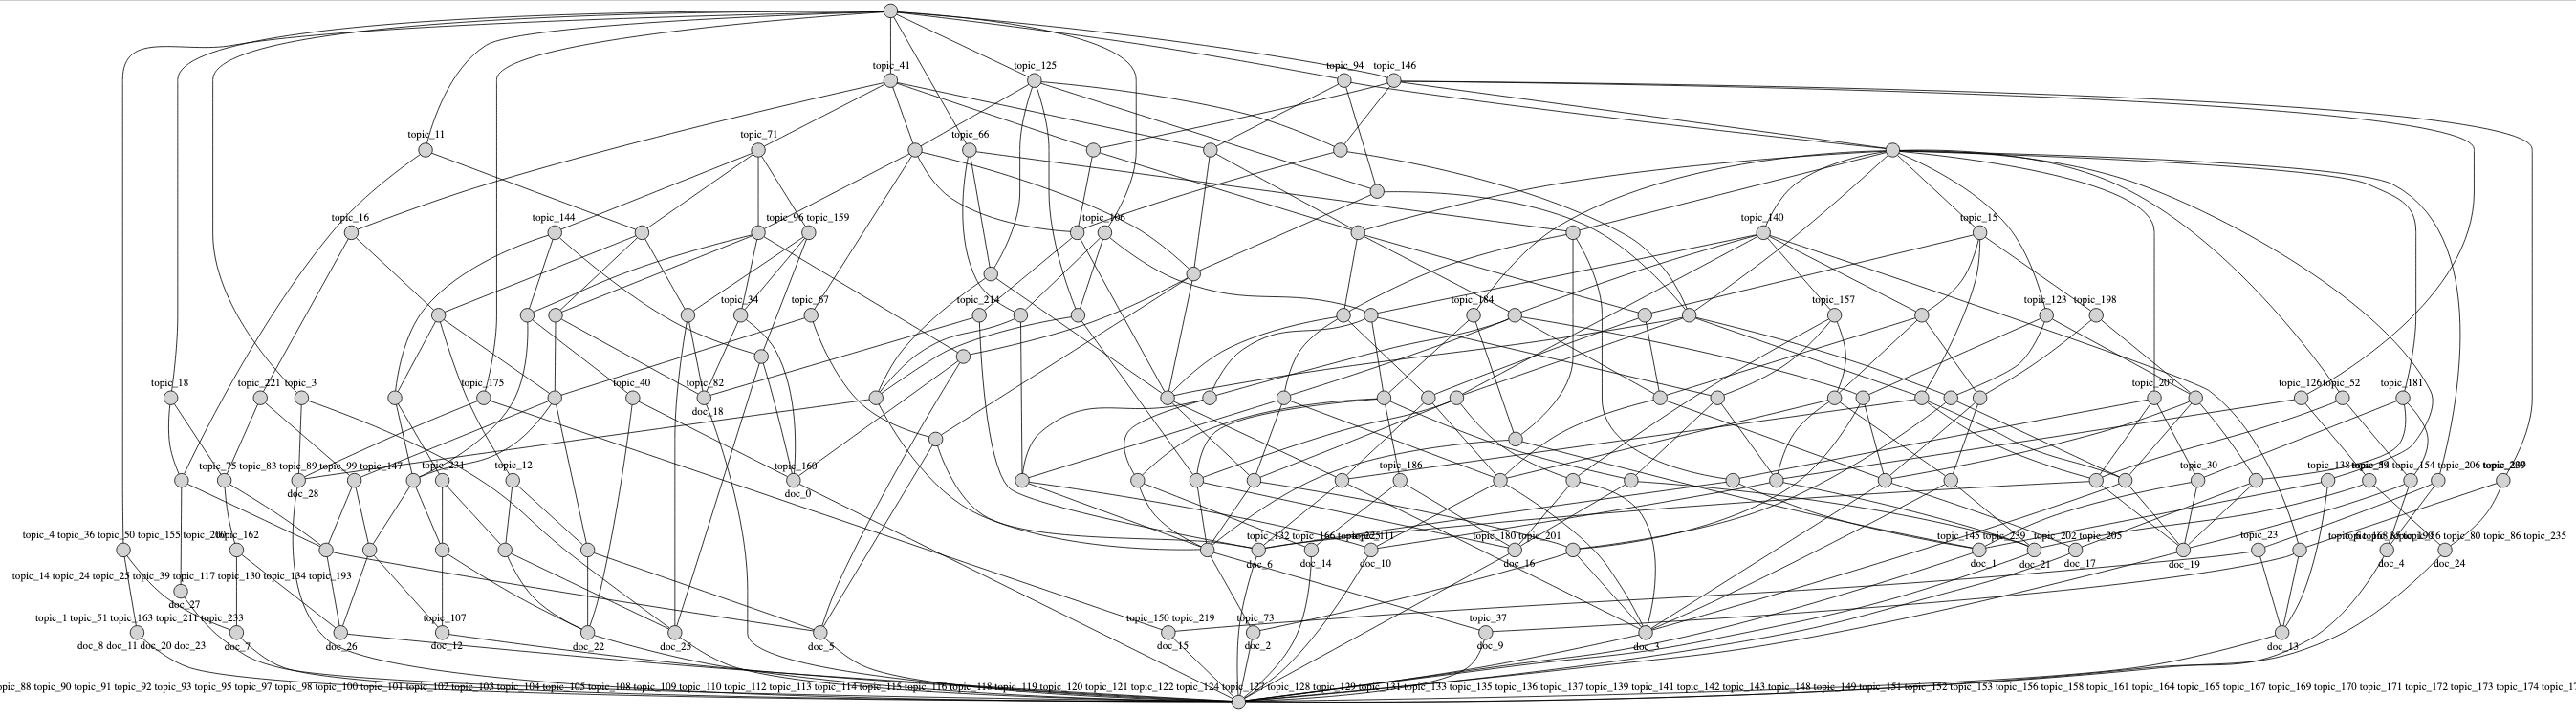
\includegraphics[width=\textwidth]{images/fca_graph_Pyrotechnics_01_28_25.png}
% }
% \only<2->{
%     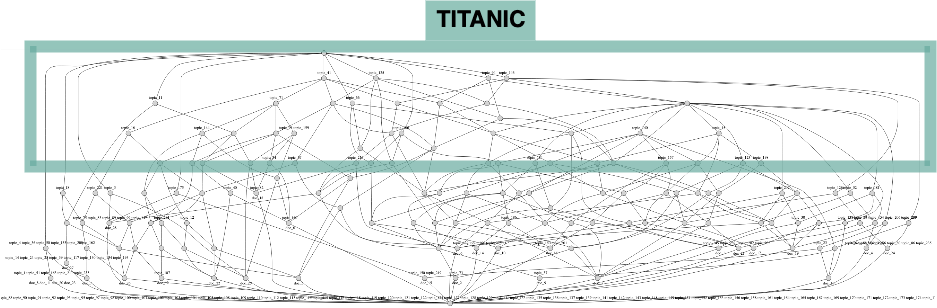
\includegraphics[width=\textwidth]{images/titanic.png}
% }


\only<1>{
\begin{figure}[htbp]
    \centering
    \resizebox{\textwidth}{!}{\FormalConceptGraph}
    \caption{Concept lattice.}
    \label{fig:titanic_formal_concept_graph}
\end{figure}
}

\only<2->{
\begin{figure}[htbp]
    \centering
    \resizebox{\textwidth}{!}{\FormalConceptGraphColoured}
    \caption{Concept lattice.}
    \label{fig:titanic_formal_concept_graph}
\end{figure}
}



\end{column}
\end{columns}
\end{frame}


\begin{frame}{TITANIC~\cite{titanic_2002}}
\begin{definition}
Support $supp(B) = \frac{\left| B' \right|}{\left| G \right|}$
\end{definition}

\begin{itemize}
    \item<2-> $minsupp \in [0,1]$ denotes minimum support threshold below which attribute sets are not considered frequent
    \item<3-> $B \subseteq M$ frequent attribute set in $\mathbb{K}$ if $supp(B) \ge minsupp$
    \item<4-> $(A, B)$ frequent concept if its intent $B$ is frequent attribute set.
\end{itemize}


\end{frame}

\begin{frame}{TITANIC~\cite{titanic_2002}}
\begin{columns}
    \begin{column}{0.7\textwidth}
        \begin{definition}
        The iceberg concept lattice of a context $\mathbb{K}$ comprises all frequent concepts.
        \end{definition}

        \only<2->{
        TITANIC algorithm computes iceberg concept lattices.
        % An iceberg concept lattice includes only the top-level concepts, specifically those corresponding to frequent attribute sets.
        }
    \end{column}
    \begin{column}{0.25\textwidth}
    \begin{figure}[htbp]
        \centering
        \resizebox{\textwidth}{!}{\FormalConceptGraphColoured}
        \caption{Iceberg concept lattice coloured.}
        \label{fig:titanic_formal_concept_graph}
    \end{figure}
    \end{column}
\end{columns}
\end{frame}